\section{Modelo}
\label{sec:modelo}

\subsection{Autómatas celulares de dos dimensiones}
\label{subsec:2d}

\subsubsection{El juego de la vida de Conway (Von Neumann)}

El Juego de la Vida de Conway es un autómata celular diseñado por el matemático británico John Horton Conway en 1970.
Es un sistema simple basado en una cuadrícula bidimensional de celdas, donde cada celda puede estar en uno de dos estados: viva o muerta.
La evolución del sistema se determina por reglas sencillas que se aplican a cada celda en función del estado de sus celdas vecinas.

Reglas:
\begin{itemize}
    \item Supervivencia: Una celda viva con 2 o 3 vecinos vivos sigue viva en la siguiente generación.

    \item Muerte por soledad: Una celda viva con menos de 2 vecinos vivos muere por soledad.

    \item Muerte por sobrepoblaión: Una celda viva con más de 3 vecinos vivos muere por sobrepoblación.

    \item Reproducción: Una celda muerta con exactamente 3 vecinos vivos "nace" (se convierte en una célula viva) en la siguiente generación.
\end{itemize}

Para esta simulación, se consideró la distancia de Von Neumann, donde una celda tiene 4 vecinos adyacentes.

\subsubsection{Vecinos impares (Moore)}

Reglas:
\begin{itemize}
    \item Si una celda tiene un número impar de vecinos vivos, en la siguiente generación estará viva
    \item Si una celda tiene un número par de vecinos vivos, en la siguiente generación estará muerta
\end{itemize}


\subsubsection{Rectángulo Relleno}
Reglas:
\begin{itemize}
    \item Una célula viva sigue viva en la siguiente generación
    \item Una célula muerta se transforma en viva si existe un par de vecinos (vecindad de moore de distancia 1) vivos que no comparten ni fila ni columna entre sí.
\end{itemize}
Entonces, en la Fig. \ref{fig:fill} se puede ver que los casos donde una celda muerta se mantiene muerta son lados rectos:
\begin{figure}[H]
    \centering
    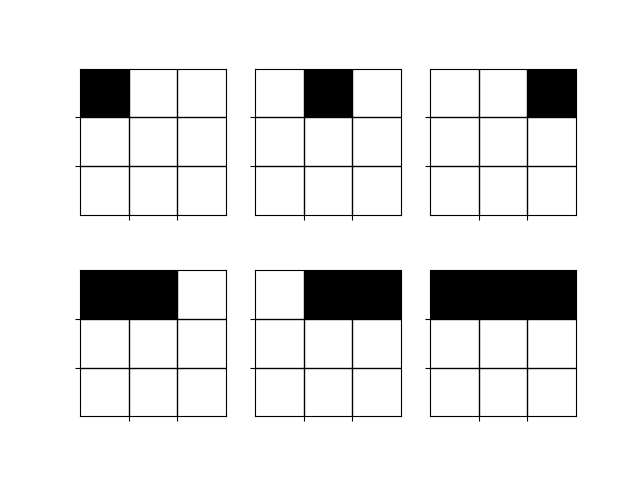
\includegraphics[width=0.5\textwidth]{Images/fill_example_1a}
    \caption{Casos donde una celda muerta se mantiene muerta}
    \label{fig:fill}
\end{figure}
Los rectángulos son las únicas superficies estables, ya que son las únicas superficies cuyo borde es exclusivamente de lados rectos, y el perímetro de celdas muertas que lo rodea cae en los casos mencionados.
Entonces, el sistema va a converger a un conjunto de rectángulos que contienen a las células vivas iniciales y estén suficientemente cerca entre sí.

\subsection{Autómatas celulares de tres dimensiones}
\label{subsec:3d}

\subsubsection{El juego de la vida de Conway 3D (Moore)}
El Juego de la Vida en 3D es una extensión tridimensional del clásico Juego de la Vida de Conway, donde en lugar de una cuadrícula bidimensional, se utiliza un espacio cúbico tridimensional.
Las reglas son las mismas que en el Juego de la Vida de Conway clásico, pero en este caso la cantidad de vecinos de cada celda será 26 en lugar de 8.

\subsubsection{Umbral (Moore)}
Reglas:
\begin{itemize}
    \item Una celda viva muere en la siguiente generación.
    \item Si una celda muerta tiene 7 o más vecinos vivos, se convierte en una celda viva en la siguiente generación.
\end{itemize}

\subsubsection{Umbral (Von Neumann)}
Similar al anterior, pero con ligeras modificaciones en las reglas para considerar la vecindad de Von Neumann.
\begin{itemize}
    \item Una celda viva muere en la siguiente generación.
    \item Si una celda muerta tiene 2 o más vecinos vivos, se convierte en una celda viva en la siguiente generación.
\end{itemize}


